
\chapter{Probability of good eviction choices with sampling\label{sec:sampling-probabilities}}

These calculations assume that our predictions are accurate -- or at the very least, that the relative ordering is accurate enough to correctly differentiate good from bad eviction candidates.

In general, let $p$ be the probability that any given buffer in the cache is optimal to evict. (or equivalently, $p$ is the fraction of the buffers in the cache which are optimal to evict)

For these calculation, we assume sampling with replacement so that multiple buffers sampled have the same probability $p$ of being optimal independently of what else was selected. For single eviction this assumption is actually true -- I do not check for duplicate samples. For multi-eviction the sampling is also with-replacement, but if the same buffer is sampled multiple times we obviously can only evict it once, and will end up evicting fewer buffers than expected. These calculations ignore this possibility, which will be very infrequent since the number of buffers is much larger than the sample size (an 8 GiB buffer pool at 8 KiB block size has a million buffers, with sample size being in the 10--100 range), so this is a very good approximation.


\section{Single eviction}

Here we select $N$ samples and evict the single best one. If any of the $N$ samples are an optimal choice we evict that one, and only evict a sub-optimal choice if none of the samples are optimal, so the probability of an optimal eviction is $1-(1-p)^N$, and the long-run expected fraction of optimal evictions is also $1-(1-p)^N$ -- assuming that $p$ stays constant and each eviction is independent, which are likely not true in general.


\section{Bulk-eviction}

Let $M$ be the number of samples selected and $k$ be the number of evictions. Note that $M=kN$ as described in Section \ref{sec:sampling-bulk-eviction}, but this does not need to be true in general.

We calculate the expected number of optimal evictions in one batch of $k$ evictions. This will depend on how many of the $M$ samples are optimal: if it is $<k$ then the number in the sample is the number which are evicted. If $\ge k$ items sampled are optimal to evict, we evict only $k$ optimal choices. The number of optimal choices from the $M$ samples follows a binomial distribution with $M$ trials and probability of success $p$. Let $P(i) = {M \choose i} p^i (1-p)^{M-i}$ be the probability that $i$ of the $M$ samples are optimal choices.

Then the expected number of optimal evictions from one batch is:
\begin{align*}
    E[\text{\# optimal evictions}] &= \sum_{i=0}^{k-1}{i\cdot P(i)} + \sum_{i=k}^{M}{k\cdot P(i)}\\ 
    &=  \sum_{i=0}^{k-1}{i\cdot P(i)} + k\left( 1-\sum_{i=0}^{k-1}{P(i)} \right)\\
    &= k + \sum_{i=0}^{k-1}(i-k)P(i)\\
    &= k - \sum_{i=0}^{k-1}{(k-i){M \choose i}p^i (1-p)^{M-i}}
\end{align*}
Note than when $M=N$ and $k=1$, this is the same as the result for single eviction.

Since we evict $k$ items at a time, the proportion of evictions which are optimal is: $1 - \sum_{i=0}^{k-1}{\left(1 - \frac{i}{k}\right) {M \choose i} p^i (1-p)^{M-i}}$

% Formatted for wolframalpha:  k - sum {(k-n) (M choose n) p^n (1-p)^(M-n)}, n=0 to k-1

Figure \ref{plot:P-opt-bulk-eviction} compares the probability of optimal eviction decisions with and without bulk eviction with a base sample size of 10. Grouping 10 evictions together improves the eviction decisions considerably, and depending on $p$ can see comparable benefits to increasing the sample size.

\begin{figure}
    \centering
    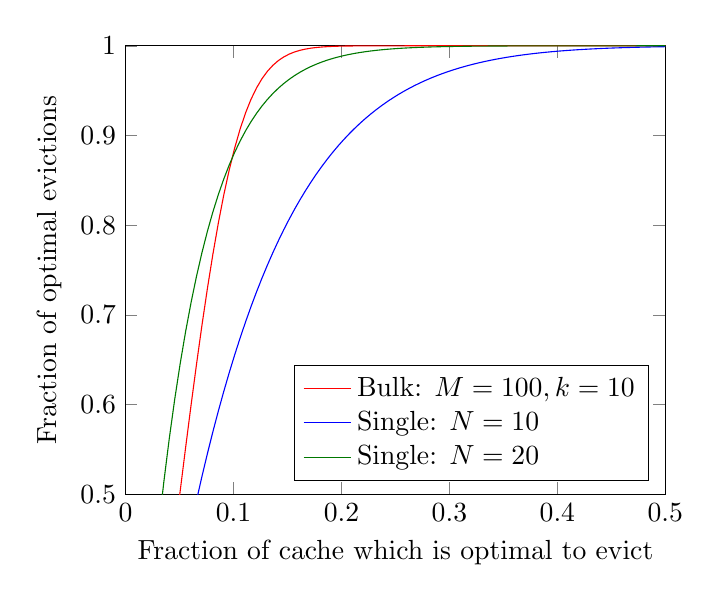
\begin{tikzpicture}
    \definecolor{darkgreen}{RGB}{0,120,0}
    \begin{axis}[
        domain=0:0.5, xmin=0, xmax=0.5,
        range=0.5:1, ymin=0.5, ymax=1,
        samples=100,
        legend pos=south east,
        legend cell align={left},
        xlabel=Fraction of cache which is optimal to evict,
        ylabel=Fraction of optimal evictions,
    ]

    \addplot[color=red]{1 - (1-x)^100 - 90 * x * (1-x)^99 - 3960 * x^2 * (1-x)^98 - 113190 * x^3 * (1-x)^97 - 2352735 * x^4 * (1-x)^96 - 37643760 * x^5 * (1-x)^95 - 476820960 * x^6 * (1-x)^94 - 4802268240 * x^7 * (1-x)^93 - 37217578860 * x^8 * (1-x)^92 - 190223180840 * x^9 * (1-x)^91)};
    % formula expanded with wolframalpha because sums and "choose" function are not available in pgfplot to my knowledge...
    \addlegendentry{Bulk: $M=100, k=10$};
    
    \addplot[color=blue]{1-(1-x)^10};
    \addlegendentry{Single: $N=10$};
    \addplot[color=darkgreen]{1-(1-x)^20};
    \addlegendentry{Single: $N=20$};
    
    \end{axis}
    \end{tikzpicture}
    \caption{Probability of an optimal eviction comparing single- vs bulk-eviction}
    \label{plot:P-opt-bulk-eviction}
\end{figure}